% Online supplement. Compiles standalone.
\documentclass[11pt]{article}
\usepackage[T1]{fontenc}
\usepackage{lmodern}
\usepackage[margin=2.8cm]{geometry}
\usepackage{amsmath,amssymb}
\usepackage{graphicx}
\graphicspath{{figs/}}
\usepackage{booktabs}
\usepackage{multirow}
% C&IE Guide for Authors: APA, seventh edition.
% Requires Biber, not BibTeX. Keep citation commands compatible with the source.
\usepackage[american]{babel}
\usepackage{csquotes}
% elsarticle 3.4 declares an unused author counter with biblatex's name.
\makeatletter
\@ifclassloaded{elsarticle}{\let\c@author\relax\let\theauthor\relax}{}
\makeatother
\usepackage[backend=biber,style=apa,natbib=true]{biblatex}
\addbibresource{ref.bib}

\newcommand{\code}[1]{\texttt{#1}}
\usepackage[hidelinks]{hyperref}
% Shared, non-identifying metadata for the manuscript and title page.
\newcommand{\PaperTitle}{Completion-aware search with partial witness repair for dense fixed-shape facility layout}
\newcommand{\TargetJournal}{Computers \& Industrial Engineering}

% Generated from the audited 60-second study; do not edit numbers by hand.

% Protocol: 3f7aac9927601181242be864ff194a933b16006cdd6b467c05f9527ff69d656a

% Result manifest: 4117224f147ee52e97fcde957de25dd4b661a22933f9d2f2cafd8331154a9d00

\newcommand{\ExtendedContrastsTable}{%
\begin{table}[htbp]
\centering
\caption{M1 minus control in percentage points of initial-objective improvement. Entries give the paired mean and descriptive pointwise 95\% interval, with equal weight for the two geometries. Positive values favor M1. Each fill 0.90 row has 20 initialized instances; fill 0.95 has 36 at $n=32$ and 40 at each other size.}
\label{tab:extendedcontrasts}
\scriptsize
\setlength{\tabcolsep}{1.5pt}
\begin{tabular}{@{}rrcccc@{}}
\toprule
$n$ & fill & \multicolumn{2}{c}{10 seconds} & \multicolumn{2}{c}{60 seconds} \\
\cmidrule(lr){3-4}\cmidrule(l){5-6}
 & & M1$-$M0 & M1$-$ALNS & M1$-$M0 & M1$-$ALNS \\
\midrule
32 & 0.90 & $-1.60\;[-3.05,-0.28]$ & $+1.01\;[-0.57,+2.52]$ & $-0.10\;[-1.22,+0.95]$ & $+0.66\;[-0.64,+2.03]$ \\
64 & 0.90 & $-1.98\;[-3.21,-0.78]$ & $+1.36\;[+0.35,+2.41]$ & $-0.79\;[-1.78,+0.18]$ & $-1.74\;[-2.76,-0.79]$ \\
128 & 0.90 & $-2.22\;[-3.84,-1.08]$ & $+5.04\;[+3.61,+6.43]$ & $-2.59\;[-3.74,-1.68]$ & $-0.41\;[-1.66,+0.88]$ \\
256 & 0.90 & $+3.98\;[+2.79,+5.25]$ & $+10.00\;[+8.98,+11.08]$ & $-4.70\;[-6.37,-3.16]$ & $+3.93\;[+2.69,+5.18]$ \\
\midrule
32 & 0.95 & $+1.35\;[+0.34,+2.28]$ & $+3.45\;[+2.47,+4.44]$ & $+1.23\;[+0.04,+2.31]$ & $+2.97\;[+2.09,+3.87]$ \\
64 & 0.95 & $-1.01\;[-2.24,+0.19]$ & $+4.16\;[+3.39,+5.01]$ & $+0.52\;[-0.57,+1.52]$ & $+1.68\;[+0.98,+2.44]$ \\
128 & 0.95 & $-0.98\;[-2.31,+0.37]$ & $+5.10\;[+4.19,+6.04]$ & $-2.35\;[-3.51,-1.20]$ & $+3.08\;[+2.33,+3.90]$ \\
256 & 0.95 & $+2.90\;[+2.08,+3.77]$ & $+5.91\;[+5.35,+6.46]$ & $-1.80\;[-2.89,-0.74]$ & $+4.12\;[+3.71,+4.54]$ \\
\bottomrule
\end{tabular}
\end{table}
}

\newcommand{\ExtendedValidationTable}{%
\begin{table}[htbp]
\centering
\caption{Validation at 10 seconds on 16 instances with two seeds. Improvement is the mean percentage gain over the common initializer. The selected ALNS configuration has removal cap four and beam width four. Candidate counts exclude the extra original position when legal; B2 and B2S use a different insertion rule.}
\label{tab:extendedvalidation}
\small
\setlength{\tabcolsep}{3pt}
\begin{tabular}{@{}lrrrr@{}}
\toprule
method & removal cap & beam width & candidates & improvement \\
\midrule
ALNS & 4 & 4 & 4 & 7.80 \\
ALNS & 8 & 4 & 4 & 7.63 \\
ALNS & 8 & 8 & 8 & 7.08 \\
ALNS & 16 & 4 & 4 & 7.15 \\
B2 & 16 & n/a & n/a & 5.83 \\
B2S & 4 & n/a & n/a & 6.99 \\
\bottomrule
\end{tabular}
\end{table}
}

\newcommand{\ExtendedCoverageTable}{%
\begin{table}[htbp]
\centering
\caption{Initialization coverage and achieved fill in the 60-second study. Failures remain in the attempted count. Fill ranges cover all attempted instances; mean initialization-attempt time is in seconds over all attempts.}
\label{tab:extendedcoverage}
\footnotesize
\setlength{\tabcolsep}{3pt}
\begin{tabular}{@{}lrrrlr@{}}
\toprule
geometry & $n$ & fill & initialized & achieved fill & init. time \\
\midrule
guillotine & 32 & 0.90 & 10/10 & 0.89815 to 0.90000 & 0.0055 \\
guillotine & 32 & 0.95 & 18/20 & 0.94318 to 0.95000 & 0.0052 \\
guillotine & 64 & 0.90 & 10/10 & 0.89855 to 0.89959 & 0.0128 \\
guillotine & 64 & 0.95 & 20/20 & 0.94792 to 0.95000 & 0.0153 \\
guillotine & 128 & 0.90 & 10/10 & 0.89938 to 0.90000 & 0.0332 \\
guillotine & 128 & 0.95 & 20/20 & 0.94885 to 0.95000 & 0.0299 \\
guillotine & 256 & 0.90 & 10/10 & 0.89965 to 0.90000 & 0.0999 \\
guillotine & 256 & 0.95 & 20/20 & 0.94943 to 0.95000 & 0.0970 \\
nonslicing & 32 & 0.90 & 10/10 & 0.89583 to 0.90000 & 0.0044 \\
nonslicing & 32 & 0.95 & 18/20 & 0.94603 to 0.95000 & 0.0036 \\
nonslicing & 64 & 0.90 & 10/10 & 0.89836 to 0.90000 & 0.0099 \\
nonslicing & 64 & 0.95 & 20/20 & 0.94796 to 0.94994 & 0.0104 \\
nonslicing & 128 & 0.90 & 10/10 & 0.89890 to 0.90000 & 0.0274 \\
nonslicing & 128 & 0.95 & 20/20 & 0.94915 to 0.95000 & 0.0304 \\
nonslicing & 256 & 0.90 & 10/10 & 0.89942 to 0.90000 & 0.0905 \\
nonslicing & 256 & 0.95 & 20/20 & 0.94933 to 0.95000 & 0.0873 \\
\bottomrule
\end{tabular}
\end{table}
}

\newcommand{\ExtendedQualityBoundaryTable}{%
\begin{table}[htbp]
\centering
\caption{Geometry-specific mean percentage improvement at fill 0.90. Seeds are averaged within each instance before the cell mean. Time excludes initialization; all methods use the common initialized set.}
\label{tab:extendedqualityboundary}
\small
\setlength{\tabcolsep}{3pt}
\begin{tabular}{@{}lrrrrr@{}}
\toprule
geometry & $n$ & seconds & M0 & M1 & ALNS \\
\midrule
guillotine & 32 & 10 & 25.08 & 21.96 & 20.00 \\
guillotine & 32 & 60 & 28.19 & 26.29 & 25.59 \\
guillotine & 64 & 10 & 17.49 & 14.80 & 12.95 \\
guillotine & 64 & 60 & 18.85 & 17.57 & 19.31 \\
guillotine & 128 & 10 & 16.20 & 14.31 & 8.52 \\
guillotine & 128 & 60 & 18.02 & 15.49 & 15.61 \\
guillotine & 256 & 10 & 8.66 & 13.44 & 3.28 \\
guillotine & 256 & 60 & 19.95 & 14.72 & 10.06 \\
\midrule
nonslicing & 32 & 10 & 18.93 & 18.86 & 18.80 \\
nonslicing & 32 & 60 & 20.67 & 22.36 & 21.75 \\
nonslicing & 64 & 10 & 16.28 & 15.01 & 14.14 \\
nonslicing & 64 & 60 & 17.70 & 17.41 & 19.14 \\
nonslicing & 128 & 10 & 17.44 & 14.89 & 10.61 \\
nonslicing & 128 & 60 & 19.63 & 16.98 & 17.68 \\
nonslicing & 256 & 10 & 10.74 & 13.93 & 4.10 \\
nonslicing & 256 & 60 & 18.84 & 14.67 & 11.47 \\
\bottomrule
\end{tabular}
\end{table}
}

\newcommand{\ExtendedQualityDenseTable}{%
\begin{table}[htbp]
\centering
\caption{Geometry-specific mean percentage improvement at fill 0.95. Seeds are averaged within each instance before the cell mean. Time excludes initialization; all methods use the common initialized set.}
\label{tab:extendedqualitydense}
\small
\setlength{\tabcolsep}{3pt}
\begin{tabular}{@{}lrrrrr@{}}
\toprule
geometry & $n$ & seconds & M0 & M1 & ALNS \\
\midrule
guillotine & 32 & 10 & 13.60 & 15.60 & 11.87 \\
guillotine & 32 & 60 & 17.72 & 19.38 & 16.25 \\
guillotine & 64 & 10 & 13.90 & 11.87 & 7.78 \\
guillotine & 64 & 60 & 16.08 & 15.90 & 13.99 \\
guillotine & 128 & 10 & 11.56 & 9.61 & 4.45 \\
guillotine & 128 & 60 & 15.50 & 12.07 & 9.14 \\
guillotine & 256 & 10 & 5.71 & 8.00 & 1.75 \\
guillotine & 256 & 60 & 11.80 & 9.12 & 4.34 \\
\midrule
nonslicing & 32 & 10 & 14.74 & 15.44 & 12.26 \\
nonslicing & 32 & 60 & 17.44 & 18.24 & 15.43 \\
nonslicing & 64 & 10 & 11.89 & 11.91 & 7.67 \\
nonslicing & 64 & 60 & 13.65 & 14.87 & 13.41 \\
nonslicing & 128 & 10 & 9.52 & 9.52 & 4.48 \\
nonslicing & 128 & 60 & 13.15 & 11.88 & 8.65 \\
nonslicing & 256 & 10 & 3.82 & 7.32 & 1.76 \\
nonslicing & 256 & 60 & 8.96 & 8.03 & 4.56 \\
\bottomrule
\end{tabular}
\end{table}
}

\newcommand{\ExtendedTargetsTable}{%
\begin{table}[htbp]
\centering
\caption{Target attainment within 60 seconds, pooling the two geometries with equal weight. Each entry is hit percentage / restricted mean search time in seconds. Non-hits contribute 60 seconds, so the time is not a success-only mean. Three seeds per instance contribute equally.}
\label{tab:extendedtargets}
\footnotesize
\setlength{\tabcolsep}{3pt}
\begin{tabular}{@{}rrlrrr@{}}
\toprule
$n$ & fill & method & target 1\% & target 5\% & target 10\% \\
\midrule
32 & 0.90 & M0 & 100.0 / 0.02 & 100.0 / 0.05 & 100.0 / 0.12 \\
32 & 0.90 & M1 & 100.0 / 0.02 & 100.0 / 0.04 & 100.0 / 0.23 \\
32 & 0.90 & ALNS & 100.0 / 0.06 & 100.0 / 0.37 & 100.0 / 1.81 \\
64 & 0.90 & M0 & 100.0 / 0.07 & 100.0 / 0.22 & 83.3 / 11.19 \\
64 & 0.90 & M1 & 100.0 / 0.05 & 100.0 / 0.51 & 95.0 / 6.15 \\
64 & 0.90 & ALNS & 100.0 / 0.16 & 100.0 / 1.69 & 95.0 / 10.23 \\
128 & 0.90 & M0 & 100.0 / 0.21 & 100.0 / 1.17 & 93.3 / 7.35 \\
128 & 0.90 & M1 & 100.0 / 0.16 & 100.0 / 0.58 & 90.0 / 7.01 \\
128 & 0.90 & ALNS & 100.0 / 0.46 & 100.0 / 3.79 & 95.0 / 16.17 \\
256 & 0.90 & M0 & 100.0 / 1.37 & 100.0 / 7.10 & 100.0 / 11.71 \\
256 & 0.90 & M1 & 100.0 / 0.64 & 100.0 / 2.58 & 100.0 / 5.30 \\
256 & 0.90 & ALNS & 100.0 / 3.01 & 96.7 / 20.55 & 53.3 / 49.75 \\
\midrule
32 & 0.95 & M0 & 100.0 / 0.06 & 100.0 / 0.65 & 88.0 / 12.76 \\
32 & 0.95 & M1 & 100.0 / 0.04 & 100.0 / 0.71 & 93.5 / 7.92 \\
32 & 0.95 & ALNS & 100.0 / 0.13 & 99.1 / 2.80 & 83.3 / 17.19 \\
64 & 0.95 & M0 & 100.0 / 0.25 & 95.8 / 4.14 & 77.5 / 18.11 \\
64 & 0.95 & M1 & 100.0 / 0.11 & 100.0 / 0.37 & 90.8 / 14.55 \\
64 & 0.95 & ALNS & 100.0 / 0.34 & 100.0 / 6.92 & 71.7 / 31.12 \\
128 & 0.95 & M0 & 100.0 / 1.87 & 94.2 / 7.48 & 72.5 / 23.71 \\
128 & 0.95 & M1 & 100.0 / 0.55 & 95.8 / 5.73 & 65.8 / 28.08 \\
128 & 0.95 & ALNS & 100.0 / 1.21 & 87.5 / 22.48 & 31.7 / 51.49 \\
256 & 0.95 & M0 & 100.0 / 4.51 & 90.0 / 20.73 & 56.7 / 39.15 \\
256 & 0.95 & M1 & 100.0 / 1.96 & 94.2 / 9.76 & 20.0 / 51.74 \\
256 & 0.95 & ALNS & 100.0 / 6.25 & 38.3 / 54.54 & 0.0 / 60.00 \\
\bottomrule
\end{tabular}
\end{table}
}

\newcommand{\ExtendedTimingTable}{%
\begin{table}[htbp]
\centering
\caption{Timing over 708 runs per method. Ratios compare process CPU time with wall time. Return overruns are milliseconds beyond the 60-second deadline. Late completed candidates are discarded, not admitted to any quality comparison. Final verification failures are zero for all methods.}
\label{tab:extendedtiming}
\scriptsize
\setlength{\tabcolsep}{3pt}
\begin{tabular}{@{}lrrrrrr@{}}
\toprule
method & mean ratio & min. ratio & median ratio & mean overrun & max. overrun & late \\
\midrule
M0 & 0.9798 & 0.6898 & 0.9970 & 5.00 & 61.06 & 42 \\
M1 & 0.9794 & 0.6953 & 0.9971 & 3.08 & 43.61 & 74 \\
ALNS & 0.9805 & 0.6515 & 0.9973 & 8.44 & 66.43 & 14 \\
\bottomrule
\end{tabular}
\end{table}
}

\hypersetup{pdfauthor={},pdftitle={Online supplement to: \PaperTitle}}

\renewcommand{\thesection}{S\arabic{section}}
\renewcommand{\thetable}{S\arabic{table}}
\renewcommand{\thefigure}{S\arabic{figure}}

\title{Online supplement to:\\
\emph{\PaperTitle}}
\ifdefined\CIEAuthorCopy
\author{Junhwan Ahn \and Kunwoo Lee \and Kyunghyun Lee \and Yeoneung Kim}
\hypersetup{pdfauthor={Junhwan Ahn, Kunwoo Lee, Kyunghyun Lee, Yeoneung Kim}}
\else
\author{}
\fi
\date{}

\begin{document}
\maketitle

\noindent This supplement contains four secondary experiments
referenced from the main text: zero shot transfer (\ref{app:transfer}),
quality and diversity fronts (\ref{app:qd}), amortized cost (\ref{app:amortize})
and action granularity (\ref{app:granularity}), followed by the full
improvement formulation ablation (\ref{app:ablation}), a qualitative
certificate gallery (\ref{app:gallery}), the complete MCNC/GSRC conversion
(\ref{app:conversion}) and the large instance feasibility record
(\ref{app:bigbench}). Each experiment follows the protocol in the main text.
These studies provide complementary diagnostics, with a relevant control for
each experiment. Section S9 gives the full budget sensitivity and
mechanism record for the comparison in which all methods start from the same
layout.
Section S10 collects additional formulation and certificate diagnostics;
complete run-level outputs remain in the archive. Sections S11 and S12 document
secondary methods, dataset coverage and policy training. Section S13 reports
the 60-second comparison of M0, M1, and ALNS, including configuration selection,
coverage, quality curves, target attainment, and timing checks.

\section{Zero shot transfer}
\label{app:transfer}
A trained policy can have an advantage through amortization. A solver restarts
for every brief, while a policy evaluates a new brief in one forward pass. We
trained a policy only on procedurally generated briefs. The type inventory,
dimensions, affinity tables, plate aspect ratio, fill ratio, wall preferences
and objective constants were randomized during $1.2$M training steps. We then
evaluated the policy on briefs that were not optimized during training.

\begin{table}[htbp]
\centering
\caption{Zero shot transfer at $n=32$. The greedy constructor provides the
direct comparison because, like the policy, it does not search over the plate.
It also requires no training. Its cost is $32$ and $528$ marginal objective
sweeps per layout; the batched figure on the heterogeneous generated set is
higher, so we report the cost for one instance.}
\label{tab:transfer}
\footnotesize
\setlength{\tabcolsep}{4pt}
\begin{tabular}{@{}lrrrrr@{}}
\toprule
 & & & \multicolumn{2}{c}{greedy constructive} & RL zero shot \\
\cmidrule(lr){4-5}
test set & shelf & SA 45k lat. & area ord. & room+pos. & ($\times16$+pol.) \\
\midrule
generated (in distribution) & 1\,912.6 & \textbf{2\,613.9} & 2\,488.8 & 2\,597.5 & 2\,591.0 \\
\textsc{office} (unseen) & 2\,942.5 & 3\,412.1 & 3\,359.5 & 3\,380.2 & \textbf{3\,426.3} \\
\textsc{clinic} (unseen) & 3\,503.7 & 4\,011.9 & 3\,955.6 & \textbf{4\,116.5} & 3\,950.2 \\
\midrule
evaluations/layout & 1 & 58\,963 to 65\,875 & 32 & 528 & 2\,049 to 5\,633 \\
\bottomrule
\end{tabular}
\end{table}

\begin{figure}[htbp]
\centering

\includegraphics[width=\linewidth]{fig_transfer.pdf}
\caption{Held out briefs, annotated with objective evaluations per layout. The
two reference scenarios were authored by hand and never optimized in training.
The RL bars show $16$ samples without the final polish ($512$ evaluations), a
cheaper operating point than the $\times16$+polish column of
Table~\ref{tab:transfer}, which is why the two differ slightly.}
\label{fig:transferapp}
\end{figure}

On \textsc{office} the zero shot policy reaches $3\,414.5$ with a single greedy
decode ($32$ evaluations, $12.7$\,ms), matching annealing's $3\,412.1$ at
$60\,371$ evaluations, and $3\,426.3$ with $16$ samples and a polish. At the same
$32$ evaluations the constructor without training reaches $3\,359.5$.

\textsc{clinic} gives a different result. The greedy constructor reaches
$4\,116.5$, which is higher than both full budget annealing and the zero shot
policy. At a matched $32$ evaluations,
it reaches $3\,955.6$ against the policy's $3\,848.5$. Across the three test sets
the zero shot policy is better on one, similar on one and worse on one. These
results show that one set of weights can evaluate unseen briefs with a quality
similar to large budget annealing while using three to four orders of magnitude
less search, with the relative ranking varying across briefs. Transfer is
evaluated at a fixed facility count
(main text, Limitations).

\section{Quality and diversity}
\label{app:qd}
A common argument for learning in design is that a policy provides a
\emph{distribution} over layouts. To compare quality and diversity across all
three methods, we vary the sampling temperature for the policy, the budget for annealing, and the
fraction of randomized commitments for the constructor without training.

\begin{table}[htbp]
\centering
\caption{Quality against diversity on \textsc{office}, $64$ samples from one
start. Diversity is the mean pairwise fraction of cells whose room type differs,
estimated from $400$ of the $2\,016$ pairs, so it carries about $\pm0.01$ of
sampling noise; every row uses the same estimator.}
\label{tab:qd}
\footnotesize
\begin{tabular}{@{}lrrr@{}}
\toprule
method & $J$ & diversity & ms/sample \\
\midrule
policy, order chosen by policy, $T{=}1.0$   & 3\,529.3 & 0.006 & 22 \\
policy, random commit order, $T{=}1.0$      & 3\,508.0 & 0.304 & 19 \\
\quad $T{=}2.5$                             & 3\,418.2 & 0.405 & 18 \\
\quad $T{=}5.0$                             & 3\,048.0 & 0.623 & 13 \\
\midrule
SA 8\,192, lattice                          & 3\,321.1 & 0.581 & 478 \\
SA 45\,000, lattice                         & 3\,414.5 & 0.639 & 1\,070 \\
\midrule
greedy constructive, area order             & 3\,359.5 & 0.000 & 7 \\
\quad $20\%$ of commit slots reshuffled     & 3\,374.5 & 0.350 & 114 \\
\quad $50\%$                                & 3\,408.3 & 0.482 & 251 \\
\quad $70\%$                                & \textbf{3\,415.2} & 0.531 & 294 \\
\quad $100\%$                               & 3\,405.2 & 0.620 & 347 \\
\bottomrule
\end{tabular}
\end{table}

\begin{figure}[htbp]
\centering

\includegraphics[width=\linewidth]{fig_qd.pdf}
\caption{Quality against diversity with all three sides swept. Faint markers are
points that a method's own front dominates.}
\label{fig:qdapp}
\end{figure}

We make three observations. First, a policy whose entropy bonus is annealed to
zero produces almost no diversity. At $T{=}1$, its diversity is $0.006$. Second,
randomizing the commit order increases diversity by a factor of fifty with a
$0.6\%$ decrease in objective. Third, applying the same procedure to the greedy
rule produces its own front. Randomizing a controlled fraction of the commit
slots changes diversity continuously from $0.000$ to $0.620$ and reaches $3\,415.2$ at
diversity $0.531$ for $32$ objective evaluations, which matches the best
annealing point anywhere on the front ($3\,414.5$ at $0.639$, $61\,267$
evaluations).

The two fronts cross once. The policy has a higher objective up to diversity
$\approx0.42$, while the constructor without training has a higher objective above
$\approx0.45$. Partial randomization of the commit order resolves the interval between
$0.000$ and $0.603$ left between the deterministic and uniformly randomized settings.
This comparison covers a single scenario; evaluation across the generated
suite remains future work.

\section{Amortized cost}
\label{app:amortize}
Training has a fixed initial cost, while search has a cost for every layout.
Table~\ref{tab:amortize} reports the annealing budget sweep on
\textsc{office}, each budget's
wall clock time per layout, and the first point on the policy's training curve
($488$ recorded checkpoints, $2\,049$\,s total) at which the policy's greedy
decode exceeds that budget's mean objective. The policy finishes at $3\,529.3$
and decodes in $17.8$\,ms per layout.

\begin{table}[htbp]
\centering
\caption{Annealing budget against the training time needed to match it. The
$45$k lattice row is the measurement of the scenario comparison (the budget
sweep's own $45$k run gives $3\,400.8$ at $1.13$\,s); the larger budgets come
from the dedicated sweep. The reference scenario implementation is not batched, so its
time per layout is omitted.}
\label{tab:amortize}
\footnotesize
\begin{tabular}{@{}lrrr@{}}
\toprule
annealer & mean $J$ & s/layout & training s to exceed \\
\midrule
non-batched reference, $45$k & 3\,269.9 & not reported & 109 \\
lattice, $45$k   & 3\,414.8 & 1.00 & 157 \\
lattice, $150$k  & 3\,459.0 & 3.40 & 215 \\
lattice, $400$k  & 3\,489.1 & 8.83 & 256 \\
lattice, $10^{6}$ & 3\,501.3 & 20.08 & 268 \\
\bottomrule
\end{tabular}
\end{table}

Charging the full $2\,049$\,s up front and $17.8$\,ms per layout thereafter,
the policy has a lower total wall clock cost than annealing with $10^{6}$
evaluations after $2049/(20.08-0.018)\approx102$ layouts. Compared with lattice
annealing using $45\,000$ evaluations, this occurs after
$2049/(1.00-0.018)\approx2\,093$ layouts.

This comparison has two limitations. First, the workload contains repeated
requests for the \emph{same} brief. An annealer could store its best layout and
reuse it for later requests. A stream of unseen briefs is evaluated separately
in \ref{app:transfer}. Second, this comparison is against annealing and not
against the constructor without training. At $88$\,ms per layout, the initial
training cost is recovered only after roughly $29\,000$ layouts relative to the
constructor. For smaller workloads, this constructor has the lower total cost.

\section{Action granularity}
\label{app:granularity}
We compare a discrete action head for small moves with a continuous displacement
head when feasibility is handled by a penalty. We report the comparison inside
the improvement MDP on the single $n=32$ \textsc{office} scenario
(best observed reward, jump and swap moves, Metropolis acceptance). One checkpoint
per action head is evaluated from the same 64 independent random starts, shown in
Table~\ref{tab:granularity}. No tradeoff appears in this evaluation. With
sampled decoding at horizon $4\,096$ the lattice head reaches $3\,069.6$ at
$50\%$ feasibility while the continuous head reaches $2\,737.0$ at $0\%$, and
deterministic decoding of either head falls into a limit cycle and loses more
than a thousand objective units. The feasible-volume record in
Table~\ref{tab:sfeasvol} explains the direction geometrically, and under the constructive
formulation the question does not arise.

\begin{table}[htbp]
\centering
\caption{Discrete against continuous action head inside the improvement MDP
with best observed reward, jump and swap moves, and Metropolis acceptance
on \textsc{office}, $n=32$: mean and standard deviation across
the same 64 independent evaluation starts.}
\label{tab:granularity}
\footnotesize
\begin{tabular}{@{}llrrr@{}}
\toprule
head & decode & horizon & $J$ & feasible \\
\midrule
discrete (lattice) & sampled & 512    & $2\,475.3\pm93.8$  & 0.00 \\
discrete (lattice) & sampled & 2\,048 & $2\,853.0\pm101.4$ & 0.06 \\
discrete (lattice) & sampled & 4\,096 & $3\,069.6\pm126.3$ & 0.50 \\
discrete (lattice) & argmax  & 4\,096 & $1\,372.6\pm228.4$ & 0.00 \\
continuous & sampled & 512    & $2\,354.7\pm76.2$  & 0.00 \\
continuous & sampled & 2\,048 & $2\,611.4\pm85.5$  & 0.00 \\
continuous & sampled & 4\,096 & $2\,737.0\pm60.8$  & 0.00 \\
continuous & mean    & 4\,096 & $1\,649.5\pm203.9$ & 0.00 \\
\bottomrule
\end{tabular}
\end{table}

\section{Improvement formulation ablation, in full}
\label{app:ablation}
The main text summarizes the improvement MDP variants on
\textsc{office}; Table~\ref{tab:ablationfull} gives every variant. Each is
trained for a matched budget of $688$k environment steps and evaluated on $64$
held out starts using stochastic decoding at $4\,096$ objective evaluations.

\begin{table}[htbp]
\centering
\caption{Improvement formulation ablation on \textsc{office}.}
\label{tab:ablationfull}
\footnotesize
\begin{tabular}{@{}llrr@{}}
\toprule
ID & configuration & $J$ & feasible \\
\midrule
A0 & reference: difference reward, translate, $\gamma{=}0.995$ & 2\,658.5 & 0\,\% \\
A0$'$ & the same with $\gamma{=}0$                              & 1\,804.3 & 0\,\% \\
A1 & \quad + best observed reward                                 & 2\,246.1 & 0\,\% \\
A2 & \quad + best observed reward, jump and swap                  & 2\,461.8 & 0\,\% \\
C1 & \quad + Metropolis accept/reject (lattice head)            & \textbf{3\,067.2} & \textbf{48\,\%} \\
C1$'$ & the same with a continuous head                         & 2\,737.0 & 0\,\% \\
\midrule
\multicolumn{2}{@{}l}{A0 evaluated deterministically (argmax)}   & 1\,445.5 & 0\,\% \\
\bottomrule
\end{tabular}
\end{table}

\section{Certificate gallery}
\label{app:gallery}
Figure~\ref{fig:gallery} shows one held out instance at fill ratio $0.95$
solved by the same largest first constructor under the four certificate
settings of the main text's certificate comparison. Without a certificate the
constructor occupies too much free space in the early steps, and the last
facilities have no legal position;
the scalar objective reports this only as a lower number.

\begin{figure}[htbp]
\centering
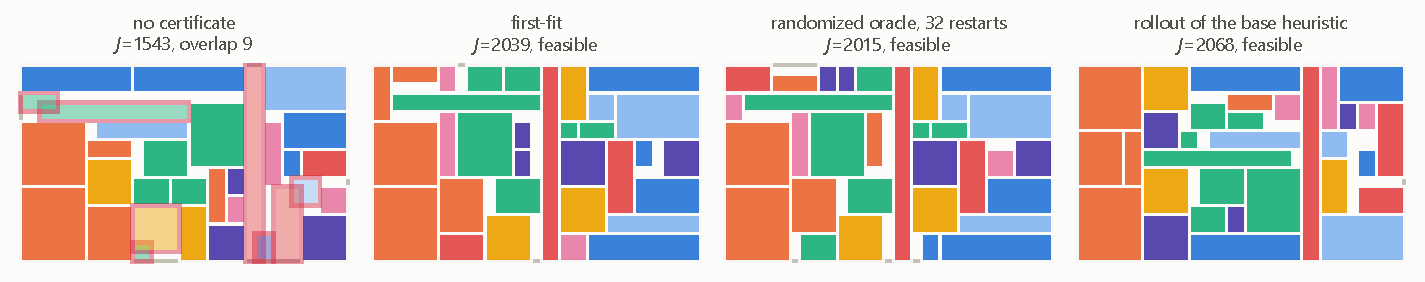
\includegraphics[width=\linewidth]{fig_gallery.pdf}
\caption{One instance, four certificates, same constructor. Facilities that
end up overlapping are outlined in red.}
\label{fig:gallery}
\end{figure}

\section{MCNC/GSRC conversion, in full}
\label{app:conversion}
HPWL numbers depend on the conversion, so we state it completely. Block
dimensions come from the GSRC \texttt{.blocks} files
(\texttt{hardrectilinear} records, width and height from the corner list);
netlists from the UCLA \texttt{.nets} files; terminal positions from the
\texttt{.pl} files, matched to net pins by name. Pins are placed at block centers and
terminals at their given coordinates, the standard simplification. Nets with
fewer than two pins are dropped, contributing zero. Coordinates are divided by
an integer for each instance and floored, which is necessary because the legality
masks are dense over the plate: the factor is $6$ for \textsc{ami33}, $33$
for \textsc{ami49} and $3$ for the GSRC instances, chosen as the smallest
divisor bringing the plate under $200$ cells per side, and it is reported with
every result. The outline is fixed by area,
$\text{plate}=\text{total block area}/(1-\text{dead space})$, at aspect
ratio $1$; blocks may be rotated by $90^\circ$. Under this conversion HPWL is
comparable across the paper's own methods but not against published
floorplanning numbers, which use full resolution and a different pin model.
Integer flooring changes block shapes and packing possibilities, so converted
dead space is not treated as a published full-resolution result.

\section{Larger-instance constructor feasibility}
\label{app:bigbench}
Table~\ref{tab:bigbench} gives the full feasibility record of the
constructors without training on $96$ to $256$ facilities summarized in the main
text. These are constructor diagnostics; M1's direct quality evaluation at
128 and 256 facilities is reported in S13.

\begin{table}[htbp]
\centering
\caption{Constructors without training on larger instances, feasibility rate.
Every instance has a verified feasible packing, so a failure indicates that the
method did not find the existing packing.
Plate geometry is drawn per cell, so methods are compared within each row.
The rollout certificate is $O(n^2WH)$ per query and was not run above
$128$ facilities.}
\label{tab:bigbench}
\footnotesize
\begin{tabular}{@{}lrccc@{}}
\toprule
$n$ & instances & no certificate & first fit & rollout \\
\midrule
\multicolumn{5}{@{}l}{\emph{fill ratio 0.85}} \\
\quad 96  & 15 & 1.00 & 1.00 & 1.00 \\
\quad 128 & 15 & 1.00 & 1.00 & 1.00 \\
\quad 192 & 15 & 1.00 & 1.00 & not run \\
\quad 256 & 15 & 1.00 & 1.00 & not run \\
\midrule
\multicolumn{5}{@{}l}{\emph{fill ratio 0.95}} \\
\quad 96  & 30 & 0.57 & 0.53 & \textbf{0.90} \\
\quad 128 & 30 & 0.53 & 0.57 & \textbf{0.90} \\
\quad 192 & 30 & 0.70 & 0.63 & not run \\
\quad 256 & 30 & 0.83 & 0.83 & not run \\
\bottomrule
\end{tabular}
\end{table}

\section{One-second mechanism study}
\label{app:sharedfull}

Every row below uses a common verified best-contact layout and retains it as a
feasible incumbent. Stochastic seeds are averaged within an instance before
cell means are computed. The 0.1 and 0.3 second values are read from the same
anytime run that continues to 1.0 second. Times exclude the common measured
initialization cost, which is charged equally to all methods in total-time
reporting. Mean initialization and verification time ranges from 0.0052 to
0.0128 seconds over the four cells. All normalized improvements use the full
feasible objective $J_\beta$, including the constant no-overlap bonus.

\begin{table}[htbp]
\centering
\caption{One-second dense study at fill 0.95. Entries are mean percentage
improvement over the common initial layout.}
\label{tab:sharedfull}
\small
\setlength{\tabcolsep}{4pt}
\begin{tabular}{@{}llrrrrrrrr@{}}
\toprule
geometry & $n$ & sec. & B1 & B2 & B2S & B3 & M0 & R0 & M1 \\
\midrule
guillotine & 32 & 0.1 & 1.72 & 0.55 & 0.82 & 2.45 & 3.50 & 1.64 & \textbf{6.14} \\
            &    & 0.3 & 1.72 & 1.22 & 1.82 & 4.37 & 7.59 & 1.96 & \textbf{7.83} \\
            &    & 1.0 & 1.72 & 2.40 & 3.51 & \textbf{9.63} & 9.04 & 2.43 & 9.51 \\
guillotine & 64 & 0.1 & 0.00 & 0.22 & 0.41 & 1.29 & \textbf{1.72} & 0.21 & 1.41 \\
            &    & 0.3 & 4.20 & 0.68 & 0.87 & 2.21 & 3.64 & 1.33 & \textbf{5.21} \\
            &    & 1.0 & 4.44 & 1.41 & 1.62 & 3.69 & 8.00 & 2.31 & \textbf{8.76} \\
nonslicing & 32 & 0.1 & 1.79 & 0.57 & 1.02 & 1.95 & 3.50 & 1.91 & \textbf{6.32} \\
            &    & 0.3 & 1.79 & 1.43 & 2.03 & 4.13 & 7.63 & 2.27 & \textbf{7.83} \\
            &    & 1.0 & 1.79 & 2.64 & 3.71 & 9.53 & \textbf{10.15} & 2.86 & 9.65 \\
nonslicing & 64 & 0.1 & 0.00 & 0.18 & 0.44 & \textbf{1.64} & 1.47 & 0.13 & 1.14 \\
            &    & 0.3 & 3.46 & 0.74 & 0.96 & 2.31 & 2.56 & 1.46 & \textbf{4.68} \\
            &    & 1.0 & 4.10 & 1.38 & 1.78 & 3.60 & 7.78 & 2.70 & \textbf{7.98} \\
\bottomrule
\end{tabular}
\end{table}

\begin{table}[htbp]
\centering
\caption{Pooled M1 minus control contrasts on 196 initialized dense instances.
Entries are percentage points with paired instance-bootstrap 95\% intervals.}
\label{tab:sharedcontrasts}
\scriptsize
\setlength{\tabcolsep}{2.4pt}
\begin{tabular}{@{}rrrrrrr@{}}
\toprule
sec. & B1 & B2 & B2S & B3 & M0 & R0 \\
\midrule
0.1 & 2.84 [2.26,3.45] & 3.32 [2.83,3.82] & 3.03 [2.56,3.52] & 1.87 [1.36,2.39] & 1.18 [0.58,1.75] & 2.75 [2.33,3.17] \\
0.3 & 3.55 [2.57,4.49] & 5.35 [4.84,5.86] & 4.95 [4.47,5.43] & 3.12 [2.58,3.67] & 1.05 [0.46,1.67] & 4.61 [4.12,5.10] \\
1.0 & 5.93 [4.99,6.88] & 7.02 [6.54,7.52] & 6.33 [5.84,6.82] & 2.41 [1.74,3.06] & 0.25 [$-0.42$,0.92] & 6.39 [5.89,6.92] \\
\bottomrule
\end{tabular}
\end{table}

At 1.0 second, the raw M1 minus B1 difference is 224.5 objective units
[172.2,276.5], its win/tie/loss count is 156/0/40, and 152 of 196 instances
exceed the one-percent practical threshold. The corresponding counts against
B2, B2S, M0 and R0 are 196/0/0, 195/0/1, 109/0/87 and 195/0/1. The M0 interval
does not establish a difference.

\begin{table}[htbp]
\centering
\caption{Boundary study at fill 0.90 and 1.0 second. Entries are mean
percentage improvement over the common initial layout. The last column is the
paired M1 minus B1 percentage-point difference with a 95\% bootstrap interval.}
\label{tab:sharedboundary}
\footnotesize
\setlength{\tabcolsep}{3.5pt}
\begin{tabular}{@{}llrrrrrrrrr@{}}
\toprule
geometry & $n$ & init. & B1 & B2 & B2S & B3 & M0 & R0 & M1 & M1$-$B1 \\
\midrule
guillotine & 32 & 20/20 & 13.03 & 7.89 & 7.60 & 8.84 & \textbf{16.17} & 7.97 & 14.60 & 1.57 [$-0.27$,3.65] \\
guillotine & 64 & 20/20 & 14.06 & 5.53 & 4.94 & 4.70 & \textbf{15.48} & 6.25 & 13.44 & $-0.62$ [$-2.09$,1.07] \\
nonslicing & 32 & 19/20 & 11.86 & 6.92 & 7.28 & 9.43 & \textbf{14.90} & 8.03 & 13.84 & 1.97 [$-0.07$,4.02] \\
nonslicing & 64 & 20/20 & 14.98 & 5.01 & 4.82 & 4.10 & \textbf{15.85} & 6.68 & 13.07 & $-1.91$ [$-3.54$,$-0.25$] \\
\bottomrule
\end{tabular}
\end{table}

\begin{table}[htbp]
\centering
\caption{Mechanism log at fill 0.95 and 1.0 second. Repair success is
conditional on a nonempty displaced set with size at most four. Verified
completions exclude the carried fallback. R0 contains reuse only, and M0 uses
full regeneration for every nonfallback proposal.}
\label{tab:repairmechanism}
\small
\begin{tabular}{@{}llrrrrrr@{}}
\toprule
geometry & $n$ & mean $|D|$ & repair success & M1 reuse & M1 verified & R0 verified & M0 verified \\
\midrule
guillotine & 32 & 1.95 & 2.45\% & 14.0 & 80.8 & 26.4 & 59.6 \\
guillotine & 64 & 2.49 & 3.91\% & 6.4 & 61.1 & 23.8 & 40.9 \\
nonslicing & 32 & 2.05 & 2.19\% & 15.9 & 76.1 & 29.7 & 59.0 \\
nonslicing & 64 & 2.72 & 3.55\% & 6.9 & 55.0 & 26.2 & 35.7 \\
\bottomrule
\end{tabular}
\end{table}

Across all dense M1 runs, the repair branch produces 6,215 incumbent updates
and 142,270 objective units of logged gain; unchanged reuse produces 1,380
updates and 12,455 units. These event counts are mechanism descriptions rather
than inferential samples. B2 and B2S have mean destroy sizes 8.88 to 9.06 and
2.99, respectively.

\begin{table}[htbp]
\centering
\caption{Mean measured work per one-second dense run, in milliseconds. Late is
the number of candidates that completed after the cutoff and were discarded.}
\label{tab:sharedtiming}
\small
\begin{tabular}{@{}lrrrrrr@{}}
\toprule
method & generation & intermediate verify & final verify & objective & return time & late \\
\midrule
B1  & 0.0 & 0.0 & 0.1 & 0.1 & 1001.53 & 0 \\
B2  & 0.0 & 0.0 & 2.9 & 2.6 & 1002.58 & 1 \\
B2S & 0.0 & 0.0 & 15.6 & 13.5 & 1002.67 & 14 \\
B3  & 845.4 & 37.7 & 40.3 & 40.9 & 1001.44 & 28 \\
M0  & 719.3 & 21.4 & 30.7 & 30.6 & 1001.26 & 23 \\
R0  & 0.0 & 12.6 & 105.0 & 92.9 & 1001.66 & 81 \\
M1  & 358.1 & 30.3 & 65.2 & 61.8 & 1001.11 & 47 \\
\bottomrule
\end{tabular}
\end{table}

All 8,820 dense budget layouts and 5,214 boundary budget layouts pass an
independent result audit. Recomputed objective and trace selection errors are
zero. No admitted dense event is later than 0.999998 seconds. Nonpreemptive
work can return up to 9.8 ms after the cutoff, but its candidate is not admitted.
The adversarial regression set rejects duplicate and missing
facilities, negative and out-of-range coordinates, overlap, stale witnesses and
incomplete timeout returns, while accepting legal edge contact.

\section{Additional formulation and certificate diagnostics}
\label{app:diagnostics}

These experiments explain the formulation and certificate choices that motivate
completion-aware construction. Table~\ref{tab:sfeasvol} shows why an overlap
penalty receives little feasible exploration as size and density increase. The
lattice column is higher than the continuous-center column wherever both are
resolved, so action representation matters before learning.

\begin{table}[htbp]
\centering
\caption{Fraction of uniformly sampled layouts that are overlap free. Each
entry averages four generated instances at $4\times10^4$ samples; $<6\times
10^{-6}$ means no feasible sample was drawn.}
\label{tab:sfeasvol}
\scriptsize
\setlength{\tabcolsep}{3pt}
\begin{tabular}{@{}lrrrrrr@{}}
\toprule
 & \multicolumn{2}{c}{fill 0.35} & \multicolumn{2}{c}{fill 0.50}
 & \multicolumn{2}{c}{fill 0.65} \\
\cmidrule(lr){2-3}\cmidrule(lr){4-5}\cmidrule(lr){6-7}
$n$ & continuous & lattice & continuous & lattice & continuous & lattice \\
\midrule
2  & $2.6\times10^{-1}$ & $3.7\times10^{-1}$ & $1.7\times10^{-1}$ & $2.4\times10^{-1}$ & $7.1\times10^{-2}$ & $1.4\times10^{-1}$ \\
4  & $3.3\times10^{-2}$ & $7.6\times10^{-2}$ & $3.0\times10^{-3}$ & $1.5\times10^{-2}$ & $5.0\times10^{-4}$ & $3.9\times10^{-3}$ \\
6  & $4.0\times10^{-3}$ & $1.7\times10^{-2}$ & $1.6\times10^{-4}$ & $1.1\times10^{-3}$ & $<6\times10^{-6}$ & $2.5\times10^{-5}$ \\
8  & $5.9\times10^{-4}$ & $4.5\times10^{-3}$ & $1.9\times10^{-5}$ & $6.9\times10^{-5}$ & $<6\times10^{-6}$ & $<6\times10^{-6}$ \\
10 & $8.8\times10^{-5}$ & $1.1\times10^{-3}$ & $<6\times10^{-6}$ & $1.3\times10^{-5}$ & $<6\times10^{-6}$ & $<6\times10^{-6}$ \\
12 & $6.3\times10^{-6}$ & $2.2\times10^{-4}$ & $<6\times10^{-6}$ & $<6\times10^{-6}$ & $<6\times10^{-6}$ & $<6\times10^{-6}$ \\
16 & $<6\times10^{-6}$ & $1.3\times10^{-5}$ & $<6\times10^{-6}$ & $<6\times10^{-6}$ & $<6\times10^{-6}$ & $<6\times10^{-6}$ \\
\bottomrule
\end{tabular}
\end{table}

The single-facility translation baseline uses the reward
$J(s_{t+1})-J(s_t)$. With discount one it optimizes the terminal objective; with
discount below one it favors high intermediate values and penalizes recovered
detours. At a common 688k-step training budget, adding a best-observed reward,
jump and swap moves, and Metropolis acceptance raised the objective from
$2\,658.5$ to $3\,067.2$ and feasibility from 0\% to 48\%. Lattice annealing
reached $3\,414.8$, and a masked constructor without training reached
$3\,380.2$. Table~\ref{tab:ablationfull} gives the complete formulation ablation.

Initialization coverage depended strongly on the witness generator. On 100-instance
dense cells $(n,f)=(32,0.90),(32,0.95),(64,0.95)$, bottom-left fill in area
order covered 0.78, 0.09 and 0.28; best-contact covered 0.98, 0.96 and 1.00.
To control for initialization, every primary method receives the same verified
best-contact layout. In the full-regeneration decoder diagnostics, the exact
marginal selector matched or exceeded the two learned selectors in most $n=64$
cells, supporting M1's use of exact marginal ranking.

Finally, the learned completion predictor was trained on 25,258 rollout states
with an instance-grouped split. Validation AUC was 0.902, but on disjoint fill
0.95 tests its best completion rate was 0.20, compared with 0.90 for verified
first fit and 1.00 for the more expensive rollout certificate. The labels record
the outcome of one heuristic rollout; membership in the set of completable
states requires a feasible continuation. These results motivate using learned
scores for candidate ordering together with independent feasibility verification.

On the two hand-authored scenarios, masked constructive search supplies most of
the improvement over translation-based search, but learning adds only 0.9\%
over the best training-free procedure in the same action set. On 60 held-out
moderate-density instances, beam search without training has the best paired
objective and solves 57, compared with 60 for the policies. These results support
the use of training-free selectors in the primary comparison; supporting tables and complete
run-level tests are reported in the Online Supplement and archive, respectively.

\section{Secondary methods and evaluation protocol}
\label{app:secondaryprotocol}
These experiments supplement the primary partial-repair comparison.

\paragraph{Design}
The suite crosses four facility counts, $n\in\{8,16,32,64\}$, with three fill
ratios, $f\in\{0.40,0.60,0.75\}$, at $20$ instances per cell: $240$ instances.
Five extensions follow the same construction from disjoint seeds.
the density diagnostic adds $f\in\{0.80,0.85,0.90,0.95\}$ at $n=32$
($80$) and $f\in\{0.85,0.90,0.95\}$ at $n=64$ ($60$);
the large-instance diagnostic adds $n\in\{96,128,192,256\}$ at $f=0.85$ and
$f=0.95$, with plates enlarged in proportion so facilities do not shrink to the
minimum size ($180$). The certified sweep also covers the $n=64,f=0.80$ cell
($20$). Finally, the frozen decoders are run on a confirmatory family of $100$
held out instances in each $n\in\{32,64\}$ by $f\in\{0.90,0.95\}$ cell ($400$), and
a small plate family at $n=8$ ($60$), sized so that constraint programming can
prove optima, supports the gap study of the main-text small-instance calibration and moderate-density diagnostic.
These diagnostic suites contain $1\,040$ distinct held out instances.
The one-second mechanism study adds 200 dense instances and 80 boundary
instances. The 60-second study adds 240 instances under distinct tags,
including 128- and 256-facility cells (S13). Every source packing is verified.
Achieved fill is recorded for each instance; integer dimensions make the target
approximate. Plate aspect ratio, types, affinities and boundary preferences vary
by instance. The randomized objective constants are drawn once per suite cell.

\paragraph{Splits}
Train, validation and test draw from disjoint generator seed ranges. Instance
identity is determined by the family, split, facility count, nominal fill,
batch size and index, together with the stored seed and tag.
The policy confirmation and the primary comparison families
use distinct generator tags. These test families are mutually disjoint and
are disjoint from training, validation and the other test cells.

\subsection{Diagnostic methods}
The matched-time methods B0 to B3, B2S, M0, R0, M1, and ALNS are defined in
the main-text method table. They are classical CPU implementations and share
the initial layout, objective, time limit and verifier. The following methods
are used in the diagnostic experiments.

\begin{itemize}
\item \textbf{Classical search}: shelf packing; lattice constrained simulated
annealing at $8\,192$ and $45\,000$ proposals; tabu search
 over single facility moves; and a lattice genetic
algorithm with uniform crossover and elitism. Annealing and tabu use periodic
greedy polish and a common budget of $45\,000$ objective calls.
Constraining annealing to the lattice is itself worth $4.4\%$ on
\textsc{office} and raises \textsc{clinic} feasibility from $20\%$ to $100\%$;
we report against this stronger version. Tabu's tenure and start and the GA's
population and memetic setting are chosen on validation like every other
hyperparameter: tabu keeps the constructive start (steepest single facility
moves cannot repair a random dense start), and the memetic variant was
rejected for exceeding the evaluation budget tenfold without improving on its
compliant counterpart.
\item \textbf{Masked constructive methods without training}: greedy with largest first
order; greedy with joint choice of facility and position; regret $k$ insertion for
$k\in\{2,4,8\}$; beam search over insertion decisions at widths $1$ to $64$; and
beam search with the order fixed to largest first.
\item \textbf{Methods without training and with certificate guidance}: largest first and joint greedy
with the certificate filter of the main-text witness construction and an argmax fallback.
These are empirical heuristics, not instances of the main-text feasible-continuation theorem.
\item \textbf{Learned}: a constructive policy trained with PPO
\citep{Schulman2017PPO}; its heuristic variant with certificate guidance; and its
full-regeneration certified variant with a carried witness. This last method uses
the invariant of the main-text feasible-continuation theorem, but not the partial repair of
the main-text partial-repair algorithm. Architecture and hyperparameters are in
\ref{app:policy}.
\end{itemize}

Beam width and regret $k$ are selected on the \emph{validation} split for the
objective comparison of the main-text small-instance calibration and moderate-density diagnostic, and the test split is
evaluated once with them fixed. The density cells of
the density diagnostic report the whole sweep instead, because the
finding there is the pattern of collapse across widths. On the two reference
scenarios, single instances with no validation counterpart, the best setting
is taken on the scenario itself; that favors the baselines without training, and
we flag it there rather than reporting a $p$ value.

\subsection{Policy coverage}
\label{sec:coverage_map}
The encoder concatenates pair features of length $n$, so one checkpoint serves one
facility count (the main-text limitations). No single policy spans the suite,
and Table~\ref{tab:datamap} states exactly which instances a learned method was
run on and which are comparisons of methods without training. Aggregate instance counts
elsewhere in the paper refer to held out \emph{test} instances; training and
validation instances are drawn from disjoint seed ranges and are not included in
the reported test aggregates.

\begin{table}[t]
\centering
\caption{Datasets, and the policies evaluated on them. Training budgets and
wall clock differ by policy family and are listed per checkpoint in
Table~\ref{tab:training} of \ref{app:policy}; training cost is per policy, not
amortized across rows.}
\label{tab:datamap}
\footnotesize
\setlength{\tabcolsep}{3pt}
\begin{tabular}{@{}llrll@{}}
\toprule
dataset & $n$ & inst. & policies & trained on \\
\midrule
generated, main    & 8, 16   & 120 & none               & not used \\
                   & 32      &  60 & 3 seeds, env order & train, $f{\le}0.75$ \\
                   & 64      &  60 & see density rows   & not used \\
generated, density & 32      &  80 & 2 seeds, own order & train, $f{=}0.75$ to $0.90$ \\
                   & 64      &  60 & 2 seeds, own order & train, $f{=}0.75$ to $0.90$ \\
generated, certified only & 64 & 20 & 2 seeds, own order & frozen; $f{=}0.80$ \\
generated, dense confirm & 32, 64 & 400 & 2 seeds, own order & frozen checkpoints \\
same initial layout, dense & 32, 64 & 200 & none & not used \\
same initial layout, boundary & 32, 64 & 80 & none & not used \\
generated, large   & 96 to 256 & 180 & none (fixed $n$)   & not used \\
generated, exact   & 8       &  60 & none               & not used \\
reference scenarios & 32     &   2 & 1 per scenario     & that scenario \\
MCNC / GSRC        & 33 to 300 &   5 & none (other obj.)  & not used \\
QAPLIB             & 12 to 30  &  32 & none (other obj.)  & not used \\
\bottomrule
\end{tabular}
\end{table}

The diagnostic experiments use the following protocol.
Every method is attempted on every instance in the cells assigned to it.
Objective comparisons are paired only on instances for which both methods return
feasible layouts. We normalize by the best \emph{feasible} objective achieved on
that instance, because raw values differ by an order of magnitude between cells
with $8$ and $64$ facilities. We report the mean paired gap, a $95\%$
bootstrap confidence interval over instances, a Wilcoxon signed rank test on
paired differences with Holm correction across the family, and the number of
instances on which each method wins. For binary reliability we report exact
binomial confidence intervals. In the prespecified dense confirmation, guided and
unfiltered decoders are paired instance by instance using the exact two sided
McNemar test, with Holm correction across all twelve selector and cell comparisons.
Coverage and feasibility conditional on return are analyzed separately for the
selective decoder.

\section{Policy and training}
\label{app:policy}
Facility tokens are embedded from features for each facility (size, placed flag,
position, boundary coefficients, and the affinity and distance rows against all
facilities) and mixed by self attention; a pointer head selects the facility.
Position selection is a fully convolutional score over the plate from dilated
residual convolutions on seven planes (occupancy, the legality mask, the affinity
of the facility being placed toward whichever facility owns each cell, the
boundary bonus it would earn, a mask for positions within bounds and two coordinate planes),
modulated channelwise by the selected facility's embedding. The encoder has no
separate embedding for each facility index, which permits transfer across briefs at
fixed $n$. The reward is the exact marginal of the main-text local marginal proposition,
so the episode return is the objective of the completed layout up to a
constant.

Unless a row of Table~\ref{tab:training} says otherwise, every constructive
policy shares one PPO configuration: $\gamma=1$, GAE $\lambda=0.95$, clip
$0.2$, Adam at $3\times10^{-4}$, $3$ epochs per batch, minibatch $512$,
value coefficient $0.5$, gradient norm clip $0.5$, entropy coefficient $0.01$
decayed linearly to zero at $80\%$ of training with a floor of $5\%$ of its
initial value, token width $128$, three attention blocks, $64$ position head
channels and $128$ parallel environments. For every policy, the final checkpoint
is used; no checkpoint selection based on validation is performed. The predictive
filter is a separate supervised diagnostic: it retains the lowest validation loss
state over $4\,000$ epochs and fixes its seven thresholds on that same grouped
validation set before any test evaluation. The five
improvement MDP checkpoints of the secondary formulation study (tabulated
in the Online Supplement, S5) are trained separately
at a matched budget of $688{,}128$ steps ($193$ to $203$\,s each). Wall clock
for policy training is on one RTX 4080 SUPER; the predictive filter was trained
on CPU in $17$\,s.

\begin{table}[t]
\centering
\caption{Training runs for the learned methods, from the stored checkpoint
histories and predictive filter metadata. Budgets end at an iteration boundary, so nominal $1.2$M
budgets record as $1{,}196{,}032$ or $1{,}198{,}080$.}
\label{tab:training}
\footnotesize
\setlength{\tabcolsep}{3pt}
\resizebox{\linewidth}{!}{%
\begin{tabular}{@{}llrrl@{}}
\toprule
policy or configuration & role & budget & min & deviations \\
\midrule
Dense-32, seeds 1/2 & density, $n=32$ & 1\,196\,032 & 34/50 & \\
Dense-64, seeds 1/2 & density, $n=64$ & 1\,196\,032 & 34/34 & \\
Suite, seeds 1/2/3 & main suite & 1\,196\,032 & 45/44/42 & random order \\
Transfer & transfer (S1) & 1\,198\,080 & 17 & 64 env, 2 ep, mb 256, 48 ch \\
Office & \textsc{office} & 1\,998\,848 & 34 & $2$M steps \\
Clinic & \textsc{clinic} & 899\,072 & 7 & $0.9$M steps, 64 env \\
\code{A0/A0'/A1/A2/C1} & improvement ablation & 688\,128 & 3.2 to 3.4 & five separate runs \\
\code{C1'} & continuous head (S4) & 688\,128 & 2.5 & continuous displacement \\
Completion predictor & predictive filter diagnostic & 4\,000 ep. & 0.28 & grouped validation \\
\bottomrule
\end{tabular}
}
\end{table}

The repository README maps these policy labels to the checkpoint files and
training histories. Seed identifiers distinguish independently trained policies;
the improvement configurations retain the identifiers used in the ablation.

\clearpage
\section{Comparison through 60 seconds}
\label{app:extended}

This study evaluates M0, M1, and an adaptive repair control on a common
initialized set. It crosses $n=32,64,128,256$, guillotine and nonslicing
geometry, and nominal fills 0.90 and 0.95, with 10 and 20 attempted instances
per geometry and size cell at the respective fills. Instance tags are disjoint
from S9, and these timing records are analyzed separately. The maximum plate
side is 44, 44, 72, and 100 for the four sizes; sampled mean-area bounds
remain 9 to 30. Integer dimensions make fill approximate. The generated
source packing is verified but withheld from every search.

\subsection{Adaptive repair control and validation}
The control is a layout-specific ALNS adaptation \citep{Ropke2006ALNS}.
It combines three removal rules with two insertion rules. Random removal
samples facilities uniformly without replacement. Spatial removal selects
facilities with centers nearest a random anchor. Low-contribution removal
ranks facilities by incident pair and boundary rewards and samples without
replacement with weights proportional to the inverse square root of rank.
The constant no-overlap bonus is omitted from these contribution scores.
The removal count is uniform from two to the selected cap.

Beam insertion visits removed facilities in decreasing area order, shuffled
with probability 0.25, and keeps a bounded frontier ranked by accumulated
exact marginal gain. Regret insertion repeatedly inserts the facility with
the largest gap between its two best legal positions, breaking ties by area.
Both use the configured number of ranked candidate positions and append the
facility's original position when legal. Every complete candidate is checked
by the same independent verifier and objective evaluator as M0 and M1.

The six operator-pair weights start at one. After an attempt, the selected
weight is updated to $\max(0.2,0.9w+0.1r)$, where the reward is six for
a new best layout, three for an accepted improving move of the current
layout, one for an accepted nonimproving move, and zero otherwise. The best
layout is retained separately from the current layout. A nonimproving move
with change $\Delta J$ is accepted with probability
$\exp(\Delta J/T)$. The initial temperature is
$0.0025\max(|J(w_0)-\beta_{\max}|,1)$ and is multiplied by 0.999 per attempt.
These online updates are fixed parts of the search rule.

Validation uses 16 disjoint instances: two per geometry, fill, and size cell
at $n=64$ and 128, with two seeds and a 10-second cutoff. The configuration
with the largest mean improvement after averaging seeds within instance is
selected before testing. Table~\ref{tab:extendedvalidation} reports all four
candidates and the B2/B2S reference controls. The selected ALNS configuration
has removal cap four, beam width four, and four ranked candidates. M0 and M1
retain $\kappa=32$, one completion attempt, and M1's repair cap of four.

\ExtendedValidationTable

\subsection{Coverage and quality}
Table~\ref{tab:extendedcoverage} includes all 240 attempted instances.
Initialization succeeds on 236; the four failures are split equally between
the two $n=32$, fill 0.95 cells and are not replaced. Three methods and three
seeds give 2,124 completed runs. Each run continues for 60 seconds and records
cutoffs 0, 0.1, 0.3, 1, 3, 10, 30, and 60 seconds.

\ExtendedCoverageTable

Tables~\ref{tab:extendedqualityboundary} and \ref{tab:extendedqualitydense}
give geometry-specific quality at the primary cutoffs. The full set of
nonzero cutoffs is shown in Figure~\ref{fig:extendedfull}. Improvement uses
$100[J_m(t)-J(w_0)]/J(w_0)$, including the constant feasible-layout bonus
in the denominator. Three seeds are averaged within each instance. Pooled
contrasts give equal weight to the two geometry families, with 10,000 paired
bootstrap samples resampling instances within geometry. All 95\% intervals
are descriptive and pointwise, without multiplicity adjustment. Raw objective
gains, every cutoff, and geometry-specific paired intervals are retained in
the accompanying result tables.

\ExtendedQualityBoundaryTable
\ExtendedQualityDenseTable

\begin{figure}[p]
\centering
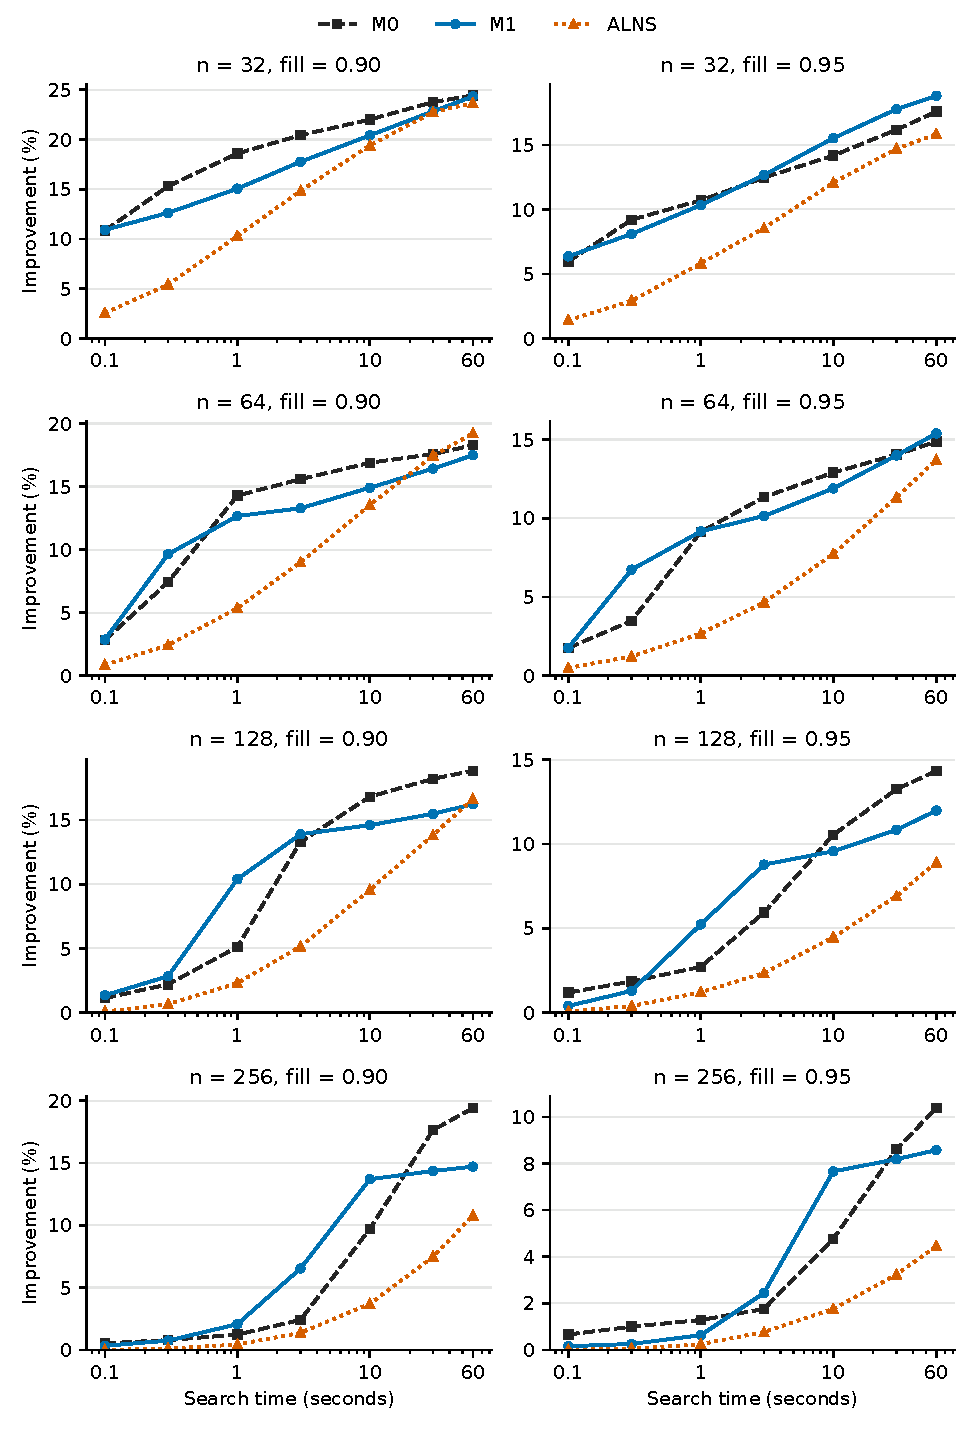
\includegraphics[width=0.94\linewidth,height=0.83\textheight,keepaspectratio]{fig_extended_anytime_full.pdf}
\caption{All size and fill cells of the 60-second comparison. Curves average
seeds within instance and then give the two geometries equal weight.
Connecting lines guide the eye between recorded cutoffs; they are not
independently restarted searches. The common initialization time is excluded.}
\label{fig:extendedfull}
\end{figure}

\subsection{Time to a target improvement}
For each run and target $q\in\{1,5,10\}\%$, the first verified trace event
reaching $q$ defines the hitting time. A non-hit contributes the 60-second
cutoff to the restricted mean. Table~\ref{tab:extendedtargets} reports both
hit percentage and restricted mean, pooling geometries equally. A companion
total-time column in the result archive adds each run's measured
initialization time. These summaries are descriptive, with equal seed counts
per instance; no success-only timing average is used.

At $n=256$, fill 0.95, M1 reaches a 5\% improvement in 94.2\% of runs with
a restricted mean of 9.76 seconds, compared with 90.0\% and 20.73 seconds
for M0. At the 10\% target, the order reverses: M0 reaches the target in
56.7\% of runs with a restricted mean of 39.15 seconds, while M1 reaches
it in 20.0\% with 51.74 seconds. This separates early moderate improvement
from attainment of a more demanding target.

\ExtendedTargetsTable

\subsection{Timing and independent checks}
Validation and test use eight single-threaded processes pinned to distinct
physical cores of an AMD Ryzen 7 9700X, with Python 3.10.18 and NumPy 2.2.5
on Windows 10. All methods and seeds for one instance run on the same core
in deterministic shuffled order. BLAS and OpenMP thread counts are one.
Table~\ref{tab:extendedtiming} reports the full-run CPU/wall ratios and return
overruns. No low-ratio run is removed. These are throughput measurements
under the stated allocation, rather than single-worker latency measurements.

\ExtendedTimingTable

The independent audit regenerates all attempted instances, checks their
source packings and common initializations, verifies all 17,228 saved layouts,
and recomputes every saved objective. It also checks the expected run identities,
trace monotonicity, and the eligibility of every saved budget row. All checks
pass, with zero objective recomputation error. The 130 completed events
finishing after the final deadline are discarded. Protocol and result-manifest
hashes link the reported tables to these audited records.

\printbibliography
\end{document}
